\documentclass{article}
\usepackage{amsmath,mathtools,geometry,pgfplots,mathrsfs,caption,wrapfig,enumitem,amssymb}
\usepackage[UTF8]{ctex}
\usetikzlibrary{arrows}
\geometry{scale=0.7}
\bibliographystyle{plain}

\title{凸多边形周长与其内部凸闭折线长度的不等关系}
\author{\kaishu 程昊一\\\kaishu{\normalsize(西安市铁一中学分校\hspace{1em}2024届励志AQ班)}}

\begin{document}
\maketitle
\paragraph{\textbf{[摘要]}\hspace{1em}}“两点之间线段最短, 这是一个最基本的命题, 由此衍生出“三角形的两边之和大于第三边”. 我们也能在生活中碰到这样的场景: 一个凸多边形包含另一个凸多边形. 此时, 两个凸多边形的周长之间应该是有一些结论的. 这篇文章, 我们列举了几种证明方法(其中一个是作者自己发现的), 并发现其中的特殊价值.
\paragraph{\textbf{[关键词]}\hspace{1em}}几何不等式\quad 闭折线的长\quad 对称性\quad 平面几何

\section{一些特殊情况}
在这一节, 我们列举了一些简单情况, 将“摘要”中描述的两个多边形化为三角形或四边形. 我们将在第二节与第三节分别证明每一个命题.

\textbf{1. }\kaishu如图\ref{fig:situation1}所示, $\triangle ABC$中有一个三角形$\triangle APC$, 则$\mathrm{C}_{\triangle ABC}$
\footnote{$\mathrm{C}_{\triangle ABC}$表示$\triangle ABC$的周长, 下同.}
与$\mathrm{C}_{\triangle APC}$之间有什么大小关系?\par
\textbf{2. }如图\ref{fig:situation2}所示, $\triangle ABC$中有一个三角形$\triangle DEF$, 则$\mathrm{C}_{\triangle ABC}$与$\mathrm{C}_{\triangle DEF}$之间有什么大小关系?\par
\textbf{3. }如图\ref{fig:situation3}所示, $\triangle ABC$中有一个四边形$ADEC$, 则$\mathrm{C}_{\triangle ABC}$与$\mathrm{C}_{\text{\songti 四边形}ADEC}$之间有什么大小关系?\par
\textbf{4. }如图\ref{fig:situation4}所示, $\triangle ABC$中有一个四边形$DEFG$, 则$\mathrm{C}_{\triangle ABC}$与$\mathrm{C}_{\text{\songti 四边形}DEFG}$之间有什么大小关系?\par
\begin{figure}[t]%4种情况
	\centering
	\begin{minipage}[c]{0.48\textwidth}
		\centering
		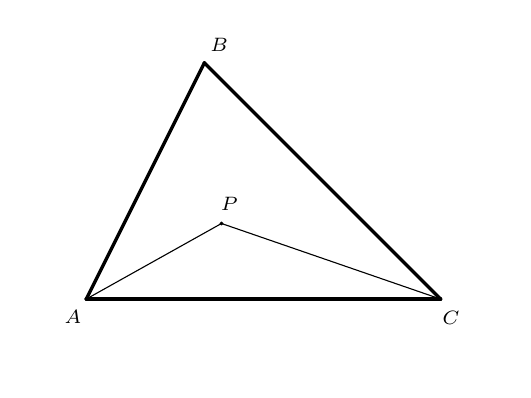
\begin{tikzpicture}[line cap=round,line join=round,>=triangle 45,x=1.5cm,y=1.5cm]%情况1
			\clip(-0.4959535919793495,-0.5993736832767338) rectangle (3.5300431861649733,2.2978090657294237);
			\draw [line width=1.2pt] (0.,0.)-- (1.,2.);
			\draw [line width=1.2pt] (1.,2.)-- (3.,0.);
			\draw [line width=1.2pt] (3.,0.)-- (0.,0.);
			\draw [line width=0.4pt] (0.,0.)-- (1.14514,0.64);
			\draw [line width=0.4pt] (1.14514,0.64)-- (3.,0.);
			\begin{scriptsize}
				\draw [fill=black] (0.,0.) circle (0.5pt);
				\draw[color=black] (-0.11222077754144746,-0.15008651303902398) node {$A$};
				\draw [fill=black] (1.,2.) circle (0.5pt);
				\draw[color=black] (1.1253175490207867,2.152310373588386) node {$B$};
				\draw [fill=black] (3.,0.) circle (0.5pt);
				\draw[color=black] (3.088750449561386,-0.1564820599463223) node {$C$};
				\draw [fill=black] (1.14514,0.64) circle (0.5pt);
				\draw[color=black] (1.2116574322693145,0.8060477496020809) node {$P$};
			\end{scriptsize}
		\end{tikzpicture}
		\caption{\kaishu 情况1}
		\label{fig:situation1}
	\end{minipage}
	\begin{minipage}[c]{0.48\textwidth}
		\centering
		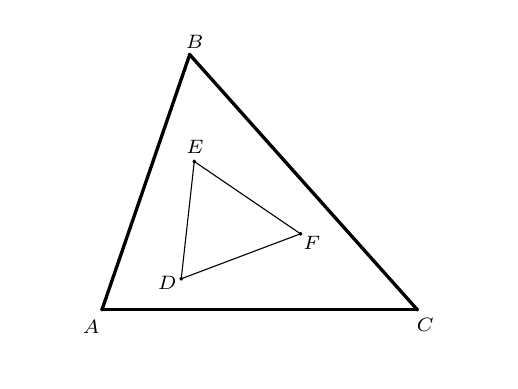
\begin{tikzpicture}[line cap=round,line join=round,>=triangle 45,x=0.75cm,y=0.75cm]%情况2
			\clip(-1.2594530243949629,-0.8690678471867949) rectangle (6.561065994718232,4.7725693931205955);
			\draw [line width=1.2pt] (0.,0.)-- (1.4843921405960117,4.31635771166581);
			\draw [line width=1.2pt] (1.4843921405960117,4.31635771166581)-- (5.3353860102502955,0.);
			\draw [line width=1.2pt] (5.3353860102502955,0.)-- (0.,0.);
			\draw [line width=0.4pt] (1.340945377542987,0.5205356739550057)-- (1.5616327053168713,2.5067216239199612);
			\draw [line width=0.4pt] (1.5616327053168713,2.5067216239199612)-- (3.36023442667403,1.2819069547749053);
			\draw [line width=0.4pt] (3.36023442667403,1.2819069547749053)-- (1.340945377542987,0.5205356739550057);
			\begin{scriptsize}
				\draw [fill=black] (0.,0.) circle (0.5pt);
				\draw[color=black] (-0.18544330906292172,-0.29194193693653125) node {$A$};
				\draw [fill=black] (1.4843921405960117,4.31635771166581) circle (0.5pt);
				\draw[color=black] (1.5675380653870763,4.528756842800965) node {$B$};
				\draw [fill=black] (5.3353860102502955,0.) circle (0.5pt);
				\draw[color=black] (5.474711340129502,-0.2672520584231509) node {$C$};
				\draw [fill=black] (1.340945377542987,0.5205356739550057) circle (0.5pt);
				\draw[color=black] (1.1046028432611965,0.4549268880932218) node {$D$};
				\draw [fill=black] (1.5616327053168713,2.5067216239199612) circle (0.5pt);
				\draw[color=black] (1.5737105350154215,2.7572580594659315) node {$E$};
				\draw [fill=black] (3.36023442667403,1.2819069547749053) circle (0.5pt);
				\draw[color=black] (3.555073285714187,1.127726077582834) node {$F$};
			\end{scriptsize}
		\end{tikzpicture}
		\caption{\kaishu 情况2}
		\label{fig:situation2}
	\end{minipage}

	\begin{minipage}[c]{0.48\textwidth}
		\centering
		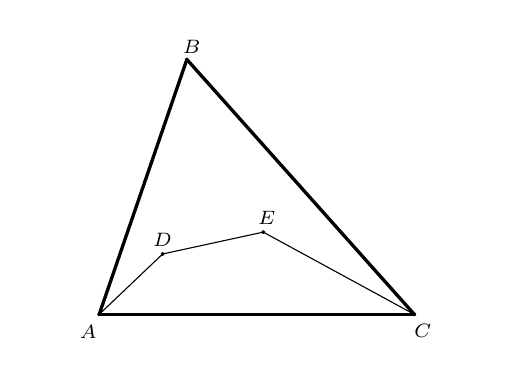
\begin{tikzpicture}[line cap=round,line join=round,>=triangle 45,x=0.75cm,y=0.75cm]%情况3
			\clip(-1.211259299755466,-0.7869413533565656) rectangle (6.609259719357729,4.85469588695083);
			\draw [line width=1.2pt] (0.,0.)-- (1.4843921405960117,4.31635771166581);
			\draw [line width=1.2pt] (1.4843921405960117,4.31635771166581)-- (5.3353860102502955,0.);
			\draw [line width=1.2pt] (5.3353860102502955,0.)-- (0.,0.);
			\draw [line width=0.4pt] (0.,0.)-- (1.0740975801392936,1.0223604906626127);
			\draw [line width=0.4pt] (1.0740975801392936,1.0223604906626127)-- (2.777699197562532,1.3927086683633165);
			\draw [line width=0.4pt] (2.777699197562532,1.3927086683633165)-- (5.3353860102502955,0.);
			\begin{scriptsize}
				\draw [fill=black] (0.,0.) circle (0.5pt);
				\draw[color=black] (-0.18662934145018567,-0.29623001790313247) node {$A$};
				\draw [fill=black] (1.4843921405960117,4.31635771166581) circle (0.5pt);
				\draw[color=black] (1.5663520329998122,4.530641231462713) node {$B$};
				\draw [fill=black] (5.3353860102502955,0.) circle (0.5pt);
				\draw[color=black] (5.479697777370582,-0.27154013938975213) node {$C$};
				\draw [fill=black] (1.0740975801392936,1.0223604906626127) circle (0.5pt);
				\draw[color=black] (1.0725544627322072,1.2654047980681706) node {$D$};
				\draw [fill=black] (2.777699197562532,1.3927086683633165) circle (0.5pt);
				\draw[color=black] (2.837880776438895,1.6295805061405297) node {$E$};
			\end{scriptsize}
		\end{tikzpicture}
		\caption{\kaishu 情况3}
		\label{fig:situation3}
	\end{minipage}
	\begin{minipage}[c]{0.48\textwidth}
		\centering
		\begin{tikzpicture}[line cap=round,line join=round,>=triangle 45,x=0.75cm,y=0.75cm]%情况4
			\clip(-2.206199679148406,-0.8389752723235143) rectangle (7.25662833397856,5.987405788448437);
			\draw [line width=1.2pt] (0.,0.)-- (1.4843921405960117,4.31635771166581);
			\draw [line width=1.2pt] (1.4843921405960117,4.31635771166581)-- (5.3353860102502955,0.);
			\draw [line width=1.2pt] (5.3353860102502955,0.)-- (0.,0.);
			\draw [line width=0.4pt] (1.3563646162435141,1.3568190732639624)-- (2.7530093190491516,1.5958170972734838);
			\draw [line width=0.4pt] (2.7530093190491516,1.5958170972734838)-- (3.4475973263268216,0.5053886127300429);
			\draw [line width=0.4pt] (3.4475973263268216,0.5053886127300429)-- (1.027742333230423,0.3709522242246871);
			\draw [line width=0.4pt] (1.027742333230423,0.3709522242246871)-- (1.3563646162435141,1.3568190732639624);
			\begin{scriptsize}
				\draw [fill=black] (0.,0.) circle (0.5pt);
				\draw[color=black] (-0.2269972928195616,-0.357244880179323) node {$A$};
				\draw [fill=black] (1.4843921405960117,4.31635771166581) circle (0.5pt);
				\draw[color=black] (1.5804252637524399,4.572089365017053) node {$B$};
				\draw [fill=black] (5.3353860102502955,0.) circle (0.5pt);
				\draw[color=black] (5.508955283408939,-0.32737012717813285) node {$C$};
				\draw [fill=black] (1.3563646162435141,1.3568190732639624) circle (0.5pt);
				\draw[color=black] (1.3563646162435141,1.651832259150715) node {$D$};
				\draw [fill=black] (2.7530093190491516,1.5958170972734838) circle (0.5pt);
				\draw[color=black] (2.827696201552127,1.883361594909939) node {$E$};
				\draw [fill=black] (3.4475973263268216,0.5053886127300429) circle (0.5pt);
				\draw[color=black] (3.679126662086045,0.27012493284567035) node {$F$};
				\draw [fill=black] (1.027742333230423,0.3709522242246871) circle (0.5pt);
				\draw[color=black] (0.773806932720307,0.20290673859299246) node {$G$};
			\end{scriptsize}
		\end{tikzpicture}
		\caption{\kaishu 情况4}
		\label{fig:situation4}
	\end{minipage}
\end{figure}
\section{一些证明的方法}
\songti 所有的方法都差不多, 均是添加辅助线, 运用“三角形两边之和大于第三边”解决问题.\par 
\begin{wrapfigure}{r}{0.45\textwidth}
	\centering
	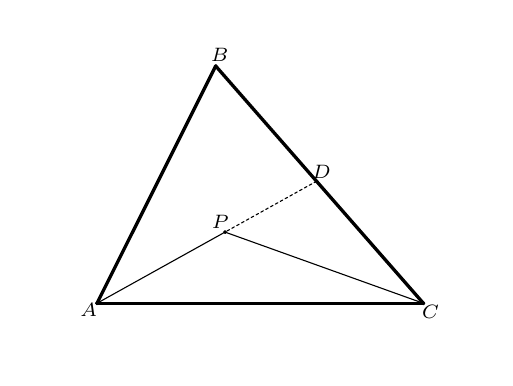
\begin{tikzpicture}[line cap=round,line join=round,>=triangle 45,x=0.8cm,y=0.8cm]
		\clip(-1.1000876631867564,-0.8627484363816061) rectangle (6.160744898936011,4.375137089885306);
		\draw [line width=1.2pt] (0.,0.)-- (1.8850155384724223,3.7660881406851594);
		\draw [line width=1.2pt] (1.8850155384724223,3.7660881406851594)-- (5.181449930577646,0.);
		\draw [line width=1.2pt] (5.181449930577646,0.)-- (0.,0.);
		\draw [line width=0.4pt] (0.,0.)-- (2.03297983626177,1.1299265956320037);
		\draw [line width=0.4pt] (2.03297983626177,1.1299265956320037)-- (5.181449930577646,0.);
		\draw [line width=0.4pt,dash pattern=on 1pt off 1pt] (3.485701799703183,1.937346892318034)-- (2.03297983626177,1.1299265956320037);
		\begin{scriptsize}
			\draw [fill=black] (0.,0.) circle (0.5pt);
			\draw[color=black] (-0.1315946063605942,-0.10915768506421115) node {$A$};
			\draw [fill=black] (1.8850155384724223,3.7660881406851594) circle (0.5pt);
			\draw[color=black] (1.9486597109642396,3.93673638664743) node {$B$};
			\draw [fill=black] (5.181449930577646,0.) circle (0.5pt);
			\draw[color=black] (5.295404948754055,-0.13208059765181251) node {$C$};
			\draw [fill=black] (2.03297983626177,1.1299265956320037) circle (0.5pt);
			\draw[color=black] (1.9601211672580403,1.2891399827794723) node {$P$};
			\draw [fill=black] (3.485701799703183,1.937346892318034) circle (0.5pt);
			\draw[color=black] (3.5647250483901436,2.0857111951986194) node {$D$};
		\end{scriptsize}
	\end{tikzpicture}
	\caption{\kaishu情况1的解答}
	\label{fig:solution1}
\end{wrapfigure}
\textbf{1. }如图\ref{fig:solution1}, 延长$AP$交$BC$于$D$. 则:
\begin{align*}
	AP+PC&<AP+(PD+DC)\\
	&=AD+DC\\
	&<(AB+BD)+DC\\
	&=AB+BC.
\end{align*}\par
所以, $AP+PC+CA<AB+BC+CA$, 即$\mathrm{C}_{\triangle ABC}\\>\mathrm{C}_{\triangle APC}$.\par
注意, 在这里, 我们实际上运用了放缩法, 在\cite{flowers}中被\\称为“切饼”. 即, 我们把$\triangle ABC$视作一张饼, 先切掉一块(在这里是$\triangle ABD$), 将$\mathrm{C}_{\triangle ABC}$放缩成$\mathrm{C}_{\triangle ADC}$; 然后, 我们再将$\triangle PDC$切掉, 只剩下所求的$\triangle APC$, 至此证明结束.\par
此证明的放缩思路是这样的:
\[\mathrm{C}_{\triangle APC}<\mathrm{C}_{\triangle ADC}<\mathrm{C}_{\triangle ABC}.\]\\\par
%%%
\textbf{2. }我们还是运用“切饼法”. \par
\begin{wrapfigure}[0]{r}[20pt]{0.45\textwidth}
	\centering
	\definecolor{uuuuuu}{rgb}{0.26666666666666666,0.26666666666666666,0.26666666666666666}
	\begin{tikzpicture}[line cap=round,line join=round,>=triangle 45,x=1.5cm,y=1.5cm]
		\clip(-0.5577830476276325,-0.4730734174119682) rectangle (3.8063536950750914,2.762792135127562);
		\draw [line width=1.2pt] (0.,0.)-- (1.0671756918782422,2.4986178993561183)-- (3.315140319816982,0.);
		\draw [line width=1.2pt] (3.315140319816982,0.)-- (0.,0.);
		\draw [line width=0.4pt] (0.8339135968876613,0.25609741056338786)-- (0.9845623995409928,1.4645628057607636)-- (2.048928940026487,0.9241921005912054);
		\draw [line width=0.4pt] (2.048928940026487,0.9241921005912054)-- (0.8339135968876613,0.25609741056338786);
		\draw [line width=0.4pt,dash pattern=on 1pt off 1pt] (0.9845623995409928,1.4645628057607636)-- (0.689504168601054,1.6143615999302705);
		\draw [line width=0.4pt,dash pattern=on 1pt off 1pt] (2.048928940026487,0.9241921005912054)-- (2.849188584339665,0.517906435016823);
		\draw [line width=0.4pt,dash pattern=on 1pt off 1pt] (0.8339135968876613,0.25609741056338786)-- (0.8019881744326048,0.);
		\begin{scriptsize}
			\draw [fill=black] (0.,0.) circle (0.5pt);
			\draw[color=black] (-0.07745353192135786,-0.09738711762741831) node {$A$};
			\draw [fill=black] (1.0671756918782422,2.4986178993561183) circle (0.5pt);
			\draw[color=black] (1.10621563178339,2.602750945664278) node {$B$};
			\draw [fill=black] (3.315140319816982,0.) circle (0.5pt);
			\draw[color=black] (3.4049354569491332,-0.0870943422908553) node {$C$};
			\draw [fill=black] (0.8339135968876613,0.25609741056338786) circle (0.5pt);
			\draw[color=black] (0.7356757196671213,0.27658371960103767) node {$D$};
			\draw [fill=black] (0.9845623995409928,1.4645628057607636) circle (0.5pt);
			\draw[color=black] (1.0581826802127627,1.5460260111104756) node {$E$};
			\draw [fill=black] (2.048928940026487,0.9241921005912054) circle (0.5pt);
			\draw[color=black] (2.084029288756878,1.0176635438335744) node {$F$};
			\draw [fill=uuuuuu] (0.689504168601054,1.6143615999302705) circle (0.5pt);
			\draw[color=uuuuuu] (0.5709913142821129,1.6935557909345453) node {$P$};
			\draw [fill=uuuuuu] (2.849188584339665,0.517906435016823) circle (0.5pt);
			\draw[color=uuuuuu] (2.931467791467234,0.5922288299223033) node {$Q$};
			\draw [fill=uuuuuu] (0.8019881744326048,0.) circle (0.5pt);
			\draw[color=uuuuuu] (0.7905705214621241,-0.10424896785179366) node {$R$};
		\end{scriptsize}
	\end{tikzpicture}
	\caption{\kaishu情况2的解答}
	\label{fig:solution2}
\end{wrapfigure}
如图\ref{fig:solution2}, 因为$PB+BQ>PQ$, 所以有 
\[\mathrm{C}_{\triangle ABC}>\mathrm{C}_{\text{四边形}APQC}.\]
这相当于我们“切掉”了$\triangle BPQ$. 我们再切掉四边形$PERA$, \\就有
\[\mathrm{C}_{\text{四边形}APQC}>\mathrm{C}_{\text{四边形}EQCR}.\]
再切掉五边形$FQCRD$, 就有
\[\mathrm{C}_{\text{五边形}FQCRD}>\mathrm{C}_{\triangle DEF}.\]\par
所以, $\mathrm{C}_{\triangle ABC}>\mathrm{C}_{\triangle DEF}.$\\\par
%%%
\textbf{3. }我们有两种思路.
\begin{enumerate}[noitemsep,label={(\arabic*)}]
	\item 如图\ref{fig:solution3.1}, 设$AD\cap CE=P$, 则$\mathrm{C}_{\text{四边形}ADEC}<\mathrm{C}_{\triangle APC}$. 于是, 我们把命题化归为“情况1”了.
	\item 如图\ref{fig:solution3.2}, 设$DE\cap AB=P$, $DE\cap CB=Q$.我们先将$\triangle BPQ$切掉, 然后分别切掉$\triangle PDA$和$\triangle QEC$.
\end{enumerate}
\begin{figure}[htbp]
	\centering
	\begin{minipage}[c]{0.48\textwidth}
		\centering
		\definecolor{uuuuuu}{rgb}{0.26666666666666666,0.26666666666666666,0.26666666666666666}
		\begin{tikzpicture}[line cap=round,line join=round,>=triangle 45,x=1.5cm,y=1.5cm]
			\clip(-0.8052538409948403,-0.5416496613570998) rectangle (4.3173957912574945,3.1392479517550274);
			\draw [line width=1.2pt] (0.,0.)-- (1.0671756918782422,2.4986178993561183)-- (3.315140319816982,0.);
			\draw [line width=1.2pt] (3.315140319816982,0.)-- (0.,0.);
			\draw [line width=0.4pt] (0.,0.)-- (0.8378601919917575,0.6262500189519996);
			\draw [line width=0.4pt] (0.8378601919917575,0.6262500189519996)-- (1.8446702612237416,0.8115030716906844);
			\draw [line width=0.4pt] (1.8446702612237416,0.8115030716906844)-- (3.315140319816982,0.);
			\draw [line width=0.4pt,dash pattern=on 1pt off 1pt] (0.8378601919917575,0.6262500189519996)-- (1.4080704636607935,1.0524478462893694);
			\draw [line width=0.4pt,dash pattern=on 1pt off 1pt] (1.4080704636607935,1.0524478462893694)-- (1.8446702612237416,0.8115030716906844);
			\begin{scriptsize}
				\draw [fill=black] (0.,0.) circle (0.5pt);
				\draw[color=black] (-0.09243231197859564,-0.11677581214120328) node {$A$};
				\draw [fill=black] (1.0671756918782422,2.4986178993561183) circle (0.5pt);
				\draw[color=black] (1.1117125308228573,2.6217475761697884) node {$B$};
				\draw [fill=black] (3.315140319816982,0.) circle (0.5pt);
				\draw[color=black] (3.4193212095025647,-0.10469409131041948) node {$C$};
				\draw [fill=black] (0.8378601919917575,0.6262500189519996) circle (0.5pt);
				\draw[color=black] (0.7975877892224782,0.7329718862905897) node {$D$};
				\draw [fill=black] (1.8446702612237416,0.8115030716906844) circle (0.5pt);
				\draw[color=black] (1.8366157806698857,0.938361140413914) node {$E$};
				\draw [fill=uuuuuu] (1.4080704636607935,1.0524478462893694) circle (0.5pt);
				\draw[color=uuuuuu] (1.4218100321463083,1.17999555702959) node {$P$};
			\end{scriptsize}
		\end{tikzpicture}
	\caption{\kaishu 情况3的第1种思路}
	\label{fig:solution3.1}
	\end{minipage}
	\begin{minipage}[c]{0.48\textwidth}
		\centering
		\definecolor{uuuuuu}{rgb}{0.26666666666666666,0.26666666666666666,0.26666666666666666}
		\begin{tikzpicture}[line cap=round,line join=round,>=triangle 45,x=1.5cm,y=1.5cm]
			\clip(-0.8052538409948403,-0.5416496613570998) rectangle (4.3173957912574945,3.1392479517550274);
			\draw [line width=1.2pt] (0.,0.)-- (1.0671756918782422,2.4986178993561183)-- (3.315140319816982,0.);
			\draw [line width=1.2pt] (3.315140319816982,0.)-- (0.,0.);
			\draw [line width=0.4pt] (0.,0.)-- (0.8378601919917575,0.6262500189519996);
			\draw [line width=0.4pt] (0.8378601919917575,0.6262500189519996)-- (1.8446702612237416,0.8115030716906844);
			\draw [line width=0.4pt] (1.8446702612237416,0.8115030716906844)-- (3.315140319816982,0.);
			\draw [line width=0.4pt,dash pattern=on 1pt off 1pt] (0.8378601919917575,0.6262500189519996)-- (0.21882707731929477,0.5123479258522667);
			\draw [line width=0.4pt,dash pattern=on 1pt off 1pt] (1.8446702612237416,0.8115030716906844)-- (2.4798893552137957,0.9283833849848544);
			\begin{scriptsize}
				\draw [fill=black] (0.,0.) circle (0.5pt);
				\draw[color=black] (-0.09243231197859564,-0.11677581214120328) node {$A$};
				\draw [fill=black] (1.0671756918782422,2.4986178993561183) circle (0.5pt);
				\draw[color=black] (1.1117125308228573,2.6217475761697884) node {$B$};
				\draw [fill=black] (3.315140319816982,0.) circle (0.5pt);
				\draw[color=black] (3.4193212095025647,-0.10469409131041948) node {$C$};
				\draw [fill=black] (0.8378601919917575,0.6262500189519996) circle (0.5pt);
				\draw[color=black] (0.7975877892224782,0.7329718862905897) node {$D$};
				\draw [fill=black] (1.8446702612237416,0.8115030716906844) circle (0.5pt);
				\draw[color=black] (1.8366157806698857,0.938361140413914) node {$E$};
				\draw [fill=uuuuuu] (0.21882707731929477,0.5123479258522667) circle (0.5pt);
				\draw[color=uuuuuu] (0.0928207407600894,0.5960457168750402) node {$P$};
				\draw [fill=uuuuuu] (2.4798893552137957,0.9283833849848544) circle (0.5pt);
				\draw[color=uuuuuu] (2.5413828291322744,1.0551511084448242) node {$Q$};
			\end{scriptsize}
		\end{tikzpicture}
	\caption{\kaishu 情况3的第2种思路}
	\label{fig:solution3.2}
	\end{minipage}
\end{figure}\par
\textbf{4. }如图\ref{fig:solution4}所示“切饼”(“切”的顺序已经由序号给出).
\begin{figure}[htbp]
	\centering
	\begin{tikzpicture}[line cap=round,line join=round,>=triangle 45,x=1.5cm,y=1.5cm]
		\clip(-0.8052538409948409,-0.5416496613570998) rectangle (4.317395791257494,3.1392479517550274);
		\draw [line width=1.2pt] (0.,0.)-- (1.0671756918782422,2.4986178993561183)-- (3.315140319816982,0.);
		\draw [line width=1.2pt] (3.315140319816982,0.)-- (0.,0.);
		\draw [line width=0.4pt] (0.8257784711609732,0.7269310258751979)-- (1.8084250987313895,0.8960751175061709);
		\draw [line width=0.4pt] (1.8084250987313895,0.8960751175061709)-- (2.2594760097473188,0.32420699818240495);
		\draw [line width=0.4pt] (2.2594760097473188,0.32420699818240495)-- (0.652607139253072,0.27185287458234186);
		\draw [line width=0.4pt] (0.652607139253072,0.27185287458234186)-- (0.8257784711609732,0.7269310258751979);
		\draw [line width=0.4pt,dash pattern=on 1pt off 1pt] (0.2695866037007152,0.6311930814763012)-- (0.8257784711609732,0.7269310258751979);
		\draw [line width=0.4pt,dash pattern=on 1pt off 1pt] (1.8084250987313895,0.8960751175061709)-- (2.415017530331945,1.00048856884725);
		\draw [line width=0.4pt,dash pattern=on 1pt off 1pt] (2.2594760097473188,0.32420699818240495)-- (2.5151885716940052,0.);
		\draw [line width=0.4pt,dash pattern=on 1pt off 1pt] (0.652607139253072,0.27185287458234186)-- (0.5491587002527116,0.);
		\draw (0.4995720087298104,0.8155303119676123) node{①};
		\draw (0.7975877892224776,0.5094600509210897) node{②};
		\draw (2.0621412361778497,0.6705496619982069) node{③};
		\draw (1.4379189932540195,0.2154715107053508) node{④};
		\begin{scriptsize}
			\draw [fill=black] (0.,0.) circle (0.5pt);
			\draw[color=black] (-0.09243231197859622,-0.11677581214120328) node {$A$};
			\draw [fill=black] (1.0671756918782422,2.4986178993561183) circle (0.5pt);
			\draw[color=black] (1.1117125308228566,2.6217475761697884) node {$B$};
			\draw [fill=black] (3.315140319816982,0.) circle (0.5pt);
			\draw[color=black] (3.4193212095025642,-0.10469409131041948) node {$C$};
			\draw [fill=black] (0.8257784711609732,0.7269310258751979) circle (0.5pt);
			\draw[color=black] (0.7855060683916939,0.833652893213788) node {$D$};
			\draw [fill=black] (1.8084250987313895,0.8960751175061709) circle (0.5pt);
			\draw[color=black] (1.8003706181775336,1.0229331862294007) node {$E$};
			\draw [fill=black] (2.2594760097473188,0.32420699818240495) circle (0.5pt);
			\draw[color=black] (2.360157016670517,0.4027381835824996) node {$F$};
			\draw [fill=black] (0.652607139253072,0.27185287458234186) circle (0.5pt);
			\draw[color=black] (0.5317899309452339,0.33427509887472473) node {$G$};
			\draw [fill=black] (0.2695866037007152,0.6311930814763012) circle (0.5pt);
			\draw[color=black] (0.16933830602171962,0.7369991265675176) node {$P$};
			\draw [fill=black] (2.415017530331945,1.00048856884725) circle (0.5pt);
			\draw[color=black] (2.5051376666399228,1.1477776348141666) node {$Q$};
			\draw [fill=black] (0.5491587002527116,0.) circle (0.5pt);
			\draw[color=black] (0.5398444114990898,-0.11274857186427534) node {$R$};
			\draw [fill=black] (2.5151885716940052,0.) circle (0.5pt);
			\draw[color=black] (2.497083186086067,-0.12885753297198707) node {$S$};
		\end{scriptsize}
	\end{tikzpicture}
	\caption{\kaishu 情况4的解答}
	\label{fig:solution4}
\end{figure}

\section{一种具有对称性的证明方法}
可以发现, 上面的证明方法都是分步完成的, 即通过一步一步地“切”掉大多边形的部分得到小多边形. 此方法易于理解, 但是有以下两点本人认为还不够完美:
\begin{enumerate}[noitemsep,label={(\arabic*)}]
	\item {\heiti 较为繁琐. }此方法未能做到“一气呵成”, 稍显繁琐.
	\item {\heiti 失去了对称性. }个人认为对称性在数学乃至学术界都是很重要的, 但此方法未能做到这一点.
\end{enumerate}\par
基于这些缺点, 本人发现了一种新的证明方法. 我们直接看最一般的命题:\par
\textbf{5. }{\kaishu如图\ref{fig:solution5}, 平面内凸$n$边形$A_1A_2\cdots A_n$($A_1$, $A_2$, $\cdots A_n$顺时针排列)中有一个凸$m$边形$B_1$$B_2$ $\cdots$$B_m$(同样, 所有点按顺时针排列). 证明:}
\[\mathrm{C}_{n\text{边形}A_1A_2\cdots A_n}<\mathrm{C}_{m\text{边形}B_1B_2\cdots B_m}.\]\par

\begin{figure}[htbp]
	\centering
	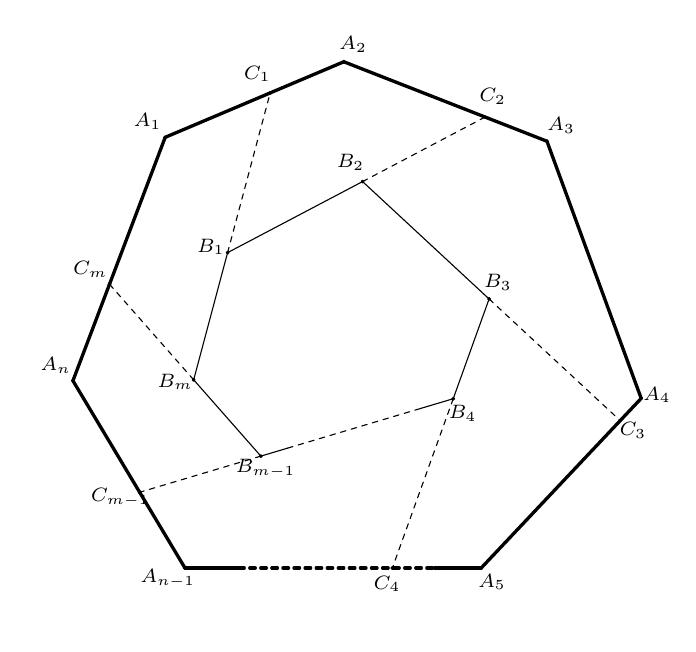
\begin{tikzpicture}[line cap=round,line join=round,>=triangle 45,x=1.2cm,y=1.2cm]
		\clip(-0.6646654021125786,-0.5896551082933829) rectangle (6.114249501662645,5.718464563130027);
		\draw [line width=1.2pt] (0.7907678220536521,4.5578569311377075)-- (2.6811106733920327,5.357617368242406);
		\draw [line width=1.2pt] (2.6811106733920327,5.357617368242406)-- (4.831116004309861,4.516310934404996);
		\draw [line width=1.2pt] (4.831116004309861,4.516310934404996)-- (5.82821992589494,1.7950481484123861);
		\draw [line width=1.2pt] (5.82821992589494,1.7950481484123861)-- (4.135220559036941,0.);
		\draw [line width=1.2pt] (1.,0.)-- (-0.18556310116507183,1.9820051337095883);
		\draw [line width=1.2pt] (-0.18556310116507183,1.9820051337095883)-- (0.7907678220536521,4.5578569311377075);
		\draw [line width=1.2pt] (1.,0.)-- (1.5683930113268802,0.);
		\draw [line width=1.2pt] (4.135220559036941,0.)-- (3.6388918093870775,0.);
		\draw [line width=1.2pt,dash pattern=on 2pt off 2pt] (1.5683930113268802,0.)-- (3.6388918093870775,0.);
		\draw [line width=0.4pt,dash pattern=on 2pt off 2pt] (1.451064746103469,3.3373909453607955)-- (1.9018784084704938,5.02794217923714);
		\draw [line width=0.4pt] (1.451064746103469,3.3373909453607955)-- (2.879708916765005,4.089672175322669);
		\draw [line width=0.4pt,dash pattern=on 2pt off 2pt] (2.879708916765005,4.089672175322669)-- (4.176436270560662,4.772489960654683);
		\draw [line width=0.4pt] (2.879708916765005,4.089672175322669)-- (4.218631472843933,2.847372896486548);
		\draw [line width=0.4pt,dash pattern=on 2pt off 2pt] (4.218631472843933,2.847372896486548)-- (5.606347192211145,1.5598016104757326);
		\draw [line width=0.4pt] (4.218631472843933,2.847372896486548)-- (3.8390400265328966,1.791418509475846);
		\draw [line width=0.4pt,dash pattern=on 2pt off 2pt] (3.8390400265328966,1.791418509475846)-- (3.1950660525383117,0.);
		\draw [line width=0.4pt,dash pattern=on 2pt off 2pt] (1.8030495417737027,1.1840721953781872)-- (0.5205706390268203,0.801502217609625);
		\draw [line width=0.4pt] (1.8030495417737027,1.1840721953781872)-- (1.0921782877730346,1.9915667266216652);
		\draw [line width=0.4pt,dash pattern=on 2pt off 2pt] (1.0921782877730346,1.9915667266216652)-- (0.20153052091680773,3.003273413244759);
		\draw [line width=0.4pt] (1.0921782877730346,1.9915667266216652)-- (1.451064746103469,3.3373909453607955);
		\draw [line width=0.4pt] (1.8030495417737027,1.1840721953781872)-- (2.085581919081345,1.2683530401343652);
		\draw [line width=0.4pt,dash pattern=on 2pt off 2pt] (2.085581919081345,1.2683530401343652)-- (3.4571024853744063,1.6774845988929743);
		\draw [line width=0.4pt] (3.4571024853744063,1.6774845988929743)-- (3.8390400265328966,1.791418509475846);
		\begin{scriptsize}
			\draw [fill=black] (0.7907678220536521,4.5578569311377075) circle (0.5pt);
			\draw[color=black] (0.6056110702288876,4.724625140061132) node {$A_1$};
			\draw [fill=black] (2.6811106733920327,5.357617368242406) circle (0.5pt);
			\draw[color=black] (2.7796348081920916,5.5390213339648104) node {$A_2$};
			\draw [fill=black] (4.831116004309861,4.516310934404996) circle (0.5pt);
			\draw[color=black] (4.981265196796098,4.683215164099928) node {$A_3$};
			\draw [fill=black] (5.82821992589494,1.7950481484123861) circle (0.5pt);
			\draw[color=black] (5.995809607845594,1.832828485437052) node {$A_4$};
			\draw [fill=black] (4.135220559036941,0.) circle (0.5pt);
			\draw[color=black] (4.24968895481483,-0.14794869804053937) node {$A_5$};
			\draw [fill=black] (1.,0.) circle (0.5pt);
			\draw[color=black] (0.8195626126951077,-0.11344038473953605) node {$A_{n-1}$};
			\draw [fill=black] (-0.18556310116507183,1.9820051337095883) circle (0.5pt);
			\draw[color=black] (-0.36752336485940384,2.143403305146082) node {$A_n$};
			\draw [fill=black] (1.451064746103469,3.3373909453607955) circle (0.5pt);
			\draw[color=black] (1.2750723482683504,3.3995059093026034) node {$B_1$};
			\draw [fill=black] (2.879708916765005,4.089672175322669) circle (0.5pt);
			\draw[color=black] (2.752028157551289,4.2898203924684895) node {$B_2$};
			\draw [fill=black] (4.218631472843933,2.847372896486548) circle (0.5pt);
			\draw[color=black] (4.3118039187566355,3.019914462991567) node {$B_3$};
			\draw [fill=black] (3.8390400265328966,1.791418509475846) circle (0.5pt);
			\draw[color=black] (3.9391141351058003,1.6395819309514335) node {$B_4$};
			\draw [fill=black] (1.8030495417737027,1.1840721953781872) circle (0.5pt);
			\draw[color=black] (1.854812011725205,1.0529406048343768) node {$B_{m-1}$};
			\draw [fill=black] (1.0921782877730346,1.9915667266216652) circle (0.5pt);
			\draw[color=black] (0.8954809019573148,1.9708617386410654) node {$B_m$};
			\draw [fill=black] (4.176436270560662,4.772489960654683) circle (0.5pt);
			\draw[color=black] (4.25659061747503,4.9937899838089574) node {$C_2$};
			\draw [fill=black] (5.606347192211145,1.5598016104757326) circle (0.5pt);
			\draw[color=black] (5.7404480894181695,1.460138701786216) node {$C_3$};
			\draw [fill=black] (3.1950660525383117,0.) circle (0.5pt);
			\draw[color=black] (3.1385212665225253,-0.1686536860211414) node {$C_4$};
			\draw [fill=black] (0.5205706390268203,0.801502217609625) circle (0.5pt);
			\draw[color=black] (0.3157412385004603,0.7423657851253467) node {$C_{m-1}$};
			\draw [fill=black] (0.20153052091680773,3.003273413244759) circle (0.5pt);
			\draw[color=black] (-0.0017352438687694774,3.15794771619558) node {$C_m$};
			\draw [fill=black] (1.9018784084704938,5.02794217923714) circle (0.5pt);
			\draw[color=black] (1.7650903971425964,5.22844651425578) node {$C_1$};
		\end{scriptsize}
	\end{tikzpicture}
	\caption{\kaishu 命题5的证明}
	\label{fig:solution5}
\end{figure}

{\heiti 证明}\quad 如图\ref{fig:solution5}, 设$B_0=B_m$, $C_0=C_m$, 延长$B_{i-1}B_i$交$n\text{边形}A_1A_2\cdots A_n$的周界(指$A_1A_2$, $A_2A_3$, $\cdots$或$A_{n-1}A_n$)于$C_1$, $C_2$, $\cdots$, $C_m$($i=$ $1$, $2$, $\cdots$, $m$). 记
\[\langle C_{i-1}, C_i\rangle\]
为$n\text{边形}A_1A_2\cdots A_n$的周界上从$C_{i-1}$到$C_i$(顺时针)的折线的长. 则由“两点之间线段最短”有如下一系列不等式:
\[\begin{cases}
	B_0C_1<B_0C_0+\langle C_0, C_1\rangle;\\
	B_1C_2<B_1C_1+\langle C_1, C_2\rangle;\\
	\hspace*{5em}\vdots\\
	B_{m-1}C_m<B_{m-1}C_{m-1}+\langle C_{m-1}, C_m\rangle;\\
\end{cases}\]
即:
\[\begin{cases}
	B_0B_1<B_0C_0+\langle C_0, C_1\rangle-B_1C_1;\\
	B_1B_2<B_1C_1+\langle C_1, C_2\rangle-B_2C_2;\\
	\hspace*{6em}\vdots\\
	B_{m-1}B_m<B_{m-1}C_{m-1}+\langle C_{m-1}, C_m\rangle-B_mC_m;\\
\end{cases}\]
将这些式子相加, 得到
\[\sum\limits_{i=1}^nB_{i-1}B_i<\sum\limits_{i=1}^n\langle C_{i-1}, C_i\rangle+\sum\limits_{i=1}^nB_{i-1}C_{i-1}-\sum\limits_{i=1}^nB_iC_i.\]\par
又显然有
\[\sum\limits_{i=1}^nB_{i-1}C_{i-1}=\sum\limits_{i=1}^nB_iC_i,\]
所以有
\[\sum\limits_{i=1}^nB_{i-1}B_i<\sum\limits_{i=1}^n\langle C_{i-1}, C_i\rangle,\]
即
\[\mathrm{C}_{n\text{边形}A_1A_2\cdots A_n}<\mathrm{C}_{m\text{边形}B_1B_2\cdots B_m}.\]
\rightline{$\square$}

\bibliography{refs}
\end{document}